\documentclass{article}
\usepackage[backend=biber,style=authoryear]{biblatex}
\usepackage{graphicx}
\usepackage{caption}
\usepackage{geometry}
\usepackage{placeins}
\usepackage{enumitem}
\usepackage{tcolorbox}
\usepackage{multirow}
\usepackage{float}
\usepackage{hyperref}
\usepackage{tabularx}
\usepackage{tikz}
\usepackage{colortbl}
\usepackage{xcolor}
\definecolor{lightgray}{RGB}{245,245,245}


\addbibresource{references.bib}

% Set page margins
\geometry{a4paper, margin=2cm}

% Set paragraph spacing
\setlength{\parindent}{0em} % No indentation
\setlength{\parskip}{0.5em} % Space between paragraphs




\begin{document}

\title{PAR - Assignment 3 - Report}
\author{\normalsize Bruno Sánchez \& Jean Dié}
\date{\small 15th December 2024}

\maketitle

\newpage
\tableofcontents
\newpage

\section{Introduction}

% Introduce the problem of designing a fuzzy expert system to detect phishing on websites. Outline the objectives and significance of the project.

\section{Task 1: Definition of Linguistic Variables}

In this task, we define the input and output linguistic variables for our fuzzy expert system designed to detect phishing on websites. Based on the features identified in \cite{Hannousse2020-eq}, we have selected a subset of five features, each with different reference scales and units, to serve as input variables. For each variable, we have determined the number of terms, labels, and corresponding fuzzy sets using trapezoidal membership function in the (a, b, c, d) format, ensuring they satisfy the property of Fuzzy Partition.


% Define the input and output linguistic variables.
% - Select a subset of five features from the literature.
% - Represent them as input linguistic variables with different scales and units.
% - Decide the number of terms, labels, and corresponding fuzzy sets.
% - Ensure the fuzzy partition property is satisfied.
% - For the output variable, define four fuzzy categories and a numerical score ranging from 0 to 100.
% - Use triangular and trapezoidal membership functions in the (a, b, c, d) format.

\subsection{Input Linguistic Variables}

For our fuzzy phishing detection system, we have carefully selected five input linguistic variables that capture key characteristics of websites commonly exploited in phishing attacks. Each variable represents a different aspect of website legitimacy, from structural elements to reputation indicators. The variables have been chosen to provide complementary signals while maintaining interpretability. We specifically selected non-binary features because binary features cannot be effectively represented using triangular or trapezoidal membership functions.

\subsubsection{Ratio of Null Hyperlinks}

This variable (f60) measures the percentage of non-functional links within a webpage, a common indicator of malicious intent. High proportions of null links often indicate hastily created phishing pages. The variable ranges from 0 to 100 percent and is characterized by three linguistic terms with trapezoidal membership functions:

\begin{table}[H]
\centering
\begin{tabularx}{\textwidth}{|>{\hsize=0.7\hsize}X|>{\hsize=0.6\hsize}X|>{\hsize=1.7\hsize}X|}
\hline
\textbf{Linguistic Term} & \textbf{Range} & \textbf{Argumentation} \\
\hline
Low & [0, 0, 10, 25] & Typical of legitimate websites with properly maintained links. A low ratio of null hyperlinks suggests that the website is well-maintained and regularly updated, reducing the likelihood of it being a phishing site. \\
\hline
Moderate & [15, 25, 35, 50] & Indicates potential suspicious activity. A moderate ratio of null hyperlinks may suggest that the website has some issues with link maintenance, which could be a sign of a less reputable site or one that is not regularly updated. \\
\hline
High & [45, 55, 100, 100] & Strong indicator of a phishing webpage. A high ratio of null hyperlinks is a red flag, as it suggests that the website may have been hastily created with little regard for link validity, a common trait of phishing sites. \\
\hline
\end{tabularx}
\caption{Linguistic Terms for Ratio of Null Hyperlinks}
\label{tab:null_hyperlinks}
\end{table}

\begin{figure}[H]
\centering
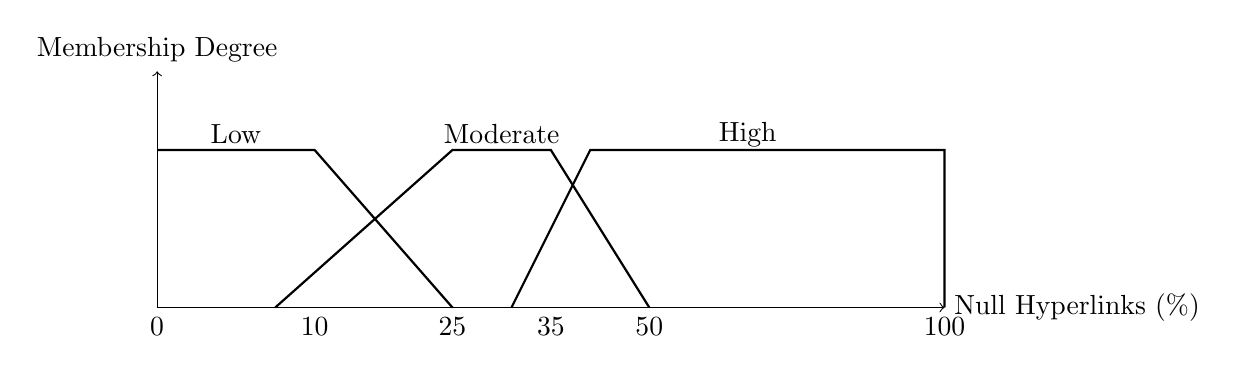
\begin{tikzpicture}
    % Axis
    \draw[->] (0,0) -- (10,0) node[right] {Null Hyperlinks (\%)};
    \draw[->] (0,0) -- (0,3) node[above] {Membership Degree};

    % Low
    \draw[thick] (0,2) -- (2,2) -- (3.75,0);
    \node at (1,2.2) {Low};

    % Moderate
    \draw[thick] (1.5,0) -- (3.75,2) -- (5,2) -- (6.25,0);
    \node at (4.375,2.2) {Moderate};

    % High
    \draw[thick] (4.5,0) -- (5.5,2) -- (10,2) -- (10,0);
    \node at (7.5,2.2) {High};

    % Labels
    \node[below] at (0,0) {0};
    \node[below] at (2,0) {10};
    \node[below] at (3.75,0) {25};
    \node[below] at (5,0) {35};
    \node[below] at (6.25,0) {50};
    \node[below] at (10,0) {100};
\end{tikzpicture}
\caption{Membership Functions for Ratio of Null Hyperlinks}
\label{fig:membership_null_hyperlinks}
\end{figure}

\subsubsection{Number of External CSS Files}

The variable f61 quantifies external stylesheet references, as legitimate websites typically maintain consistent styling through multiple CSS files. The range spans from 0 to 20 files, with three linguistic terms:

\begin{table}[H]
\centering
\begin{tabularx}{\textwidth}{|>{\hsize=0.7\hsize}X|>{\hsize=0.6\hsize}X|>{\hsize=1.7\hsize}X|}
\hline
\textbf{Linguistic Term} & \textbf{Range} & \textbf{Argumentation} \\
\hline
Very Few & [0, 0, 1, 2] & Common in phishing sites that employ minimal styling to create basic replicas of legitimate pages. A single CSS file often indicates oversimplified implementation that warrants scrutiny. \\
\hline
Moderate & [1, 2, 3, 4] & Represents balanced styling implementation. This range aligns with modern web development practices where CSS is modular but optimized for performance. \\
\hline
Normal & [3, 4, 8, 8] & Characteristic of properly developed sites with comprehensive styling needs. The upper limit reflects current best practices in CSS organization while acknowledging that excessive CSS files may indicate poor optimization. \\
\hline
\end{tabularx}
\caption{Linguistic Terms for Number of External CSS Files}
\label{tab:css_files}
\end{table}

\begin{figure}[H]
\centering
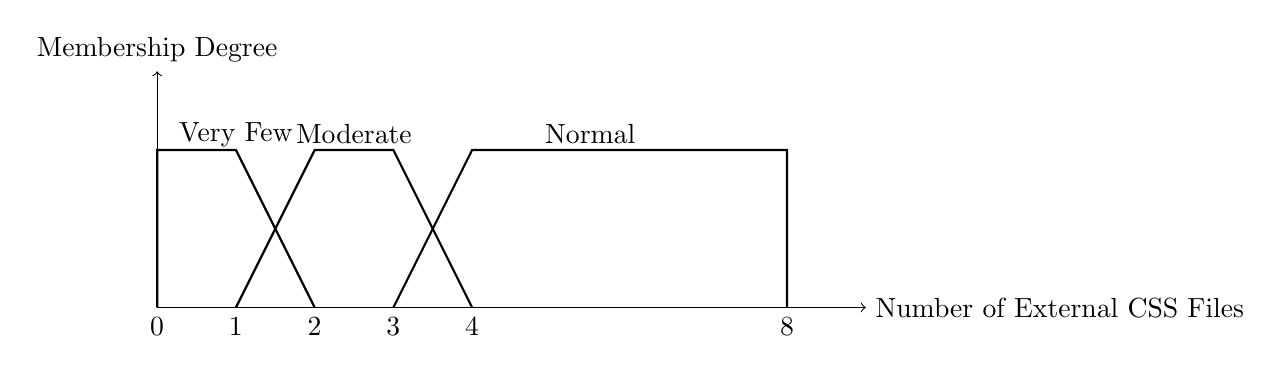
\begin{tikzpicture}
    % Axis
    \draw[->] (0,0) -- (9,0) node[right] {Number of External CSS Files};
    \draw[->] (0,0) -- (0,3) node[above] {Membership Degree};

    % Very Few
    \draw[thick] (0,0) -- (0,2) -- (1,2) -- (2,0);
    \node at (1,2.2) {Very Few};

    % Moderate
    \draw[thick] (1,0) -- (2,2) -- (3,2) -- (4,0);
    \node at (2.5,2.2) {Moderate};

    % Normal
    \draw[thick] (3,0) -- (4,2) -- (8,2) -- (8,0);
    \node at (5.5,2.2) {Normal};

    % Labels
    \node[below] at (0,0) {0};
    \node[below] at (1,0) {1};
    \node[below] at (2,0) {2};
    \node[below] at (3,0) {3};
    \node[below] at (4,0) {4};
    \node[below] at (8,0) {8};
\end{tikzpicture}
\caption{Membership Functions for Number of External CSS Files}
\label{fig:membership_css_files}
\end{figure}
    
\subsubsection{Domain Registration Length}

This variable (f82) reflects the duration of domain registration in years, as phishing sites often use short-term registrations. The range spans 1 to 10 years and is characterized by three linguistic terms with trapezoidal membership functions:

\begin{table}[H]
\centering
\begin{tabularx}{\textwidth}{|>{\hsize=0.7\hsize}X|>{\hsize=0.6\hsize}X|>{\hsize=1.7\hsize}X|}
\hline
\textbf{Linguistic Term} & \textbf{Range} & \textbf{Argumentation} \\
\hline
Short & [1, 1, 2, 3] & Common for phishing domains. Short registration lengths are often used by phishing sites to avoid detection and minimize costs. \\
\hline
Medium & [2, 3, 5, 7] & Moderate commitment to domain maintenance. Medium registration lengths may indicate a more established site, but not necessarily a highly reputable one. \\
\hline
Long & [5, 7, 10, 10] & Typical of established legitimate websites. Long registration lengths suggest a strong commitment to maintaining the domain, which is characteristic of legitimate websites. \\
\hline
\end{tabularx}
\caption{Linguistic Terms for Domain Registration Length}
\label{tab:domain_registration_length}
\end{table}

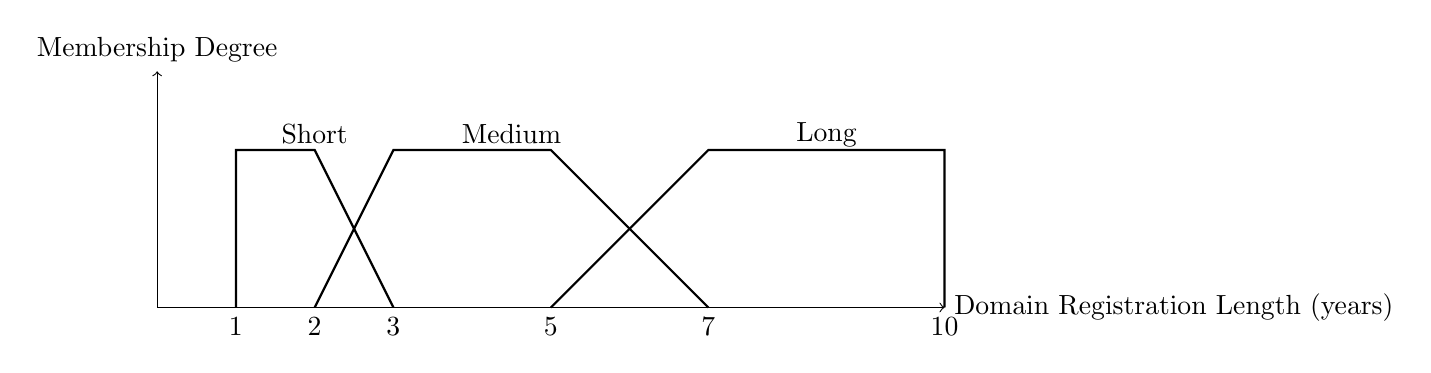
\begin{tikzpicture}
    % Axis
    \draw[->] (0,0) -- (10,0) node[right] {Domain Registration Length (years)};
    \draw[->] (0,0) -- (0,3) node[above] {Membership Degree};

    % Short
    \draw[thick] (1,0) -- (1,2) -- (2,2) -- (3,0);
    \node at (2,2.2) {Short};

    % Medium
    \draw[thick] (2,0) -- (3,2) -- (5,2) -- (7,0);
    \node at (4.5,2.2) {Medium};

    % Long
    \draw[thick] (5,0) -- (7,2) -- (10,2) -- (10,0);
    \node at (8.5,2.2) {Long};

    % Labels
    \node[below] at (1,0) {1};
    \node[below] at (2,0) {2};
    \node[below] at (3,0) {3};
    \node[below] at (5,0) {5};
    \node[below] at (7,0) {7};
    \node[below] at (10,0) {10};
\end{tikzpicture}

\subsubsection{Web Traffic}

This variable (f84) measures the percentile rank of a website's traffic, as higher traffic is typically associated with more reputable sites. The range spans from 0 to 100 percentiles and is characterized by four linguistic terms with trapezoidal membership functions:

\begin{table}[H]
\centering
\begin{tabularx}{\textwidth}{|>{\hsize=0.7\hsize}X|>{\hsize=0.6\hsize}X|>{\hsize=1.7\hsize}X|}
\hline
\textbf{Linguistic Term} & \textbf{Range} & \textbf{Argumentation} \\
\hline
Very Low & [0, 0, 10, 20] & Indicative of low visibility and potential risk. Websites with very low traffic are less likely to be well-known and may be newly created or less reputable. \\
\hline
Low & [10, 20, 60, 70] & Suggests limited reach and moderate risk. Low traffic websites may be legitimate but are not widely recognized, which can be a characteristic of less established sites. \\
\hline
Moderate & [60, 70, 80, 90] & Represents average visibility and lower risk. Moderate traffic websites are more likely to be established and have a consistent user base, indicating a higher likelihood of legitimacy. \\
\hline
High & [80, 90, 100, 100] & Characteristic of popular and reputable websites. High traffic websites are well-known and widely visited, reducing the likelihood of them being phishing sites. \\
\hline
\end{tabularx}
\caption{Linguistic Terms for Web Traffic}
\label{tab:web_traffic}
\end{table}

\begin{figure}[H]
\centering
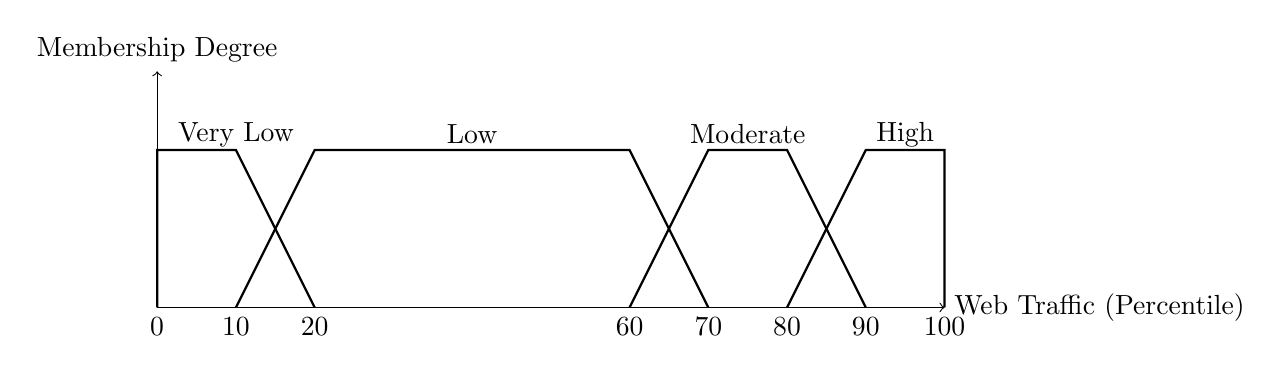
\begin{tikzpicture}
    % Axis
    \draw[->] (0,0) -- (10,0) node[right] {Web Traffic (Percentile)};
    \draw[->] (0,0) -- (0,3) node[above] {Membership Degree};

    % Very Low
    \draw[thick] (0,0) -- (0,2) -- (1,2) -- (2,0);
    \node at (1,2.2) {Very Low};

    % Low
    \draw[thick] (1,0) -- (2,2) -- (6,2) -- (7,0);
    \node at (4,2.2) {Low};

    % Moderate
    \draw[thick] (6,0) -- (7,2) -- (8,2) -- (9,0);
    \node at (7.5,2.2) {Moderate};

    % High
    \draw[thick] (8,0) -- (9,2) -- (10,2) -- (10,0);
    \node at (9.5,2.2) {High};

    % Labels
    \node[below] at (0,0) {0};
    \node[below] at (1,0) {10};
    \node[below] at (2,0) {20};
    \node[below] at (6,0) {60};
    \node[below] at (7,0) {70};
    \node[below] at (8,0) {80};
    \node[below] at (9,0) {90};
    \node[below] at (10,0) {100};
\end{tikzpicture}
\caption{Membership Functions for Web Traffic}
\label{fig:membership_web_traffic}
\end{figure}

\subsubsection{Page Rank}

This variable (f87) measures the popularity score of a website, ranging from 0 to 10. Higher page ranks are typically associated with more reputable and well-known websites. The range spans from 0 to 10 and is characterized by three linguistic terms with trapezoidal membership functions:

\begin{table}[H]
\centering
\begin{tabularx}{\textwidth}{|>{\hsize=0.7\hsize}X|>{\hsize=0.6\hsize}X|>{\hsize=1.7\hsize}X|}
\hline
\textbf{Linguistic Term} & \textbf{Range} & \textbf{Argumentation} \\
\hline
Popular & [0, 0, 2, 3] & Indicative of highly reputable websites. A high page rank suggests that the website is well-known and widely trusted, reducing the likelihood of it being a phishing site. \\
\hline
Moderately Known & [2, 3, 5, 7] & Represents websites with moderate popularity. These sites are somewhat known and trusted, but not as widely recognized as those with higher page ranks. \\
\hline
Not Very Known & [5, 7, 10, 10] & Characteristic of less reputable websites. A low page rank indicates that the website is not widely known or trusted, which could be a sign of a phishing site. \\
\hline
\end{tabularx}
\caption{Linguistic Terms for Page Rank}
\label{tab:page_rank}
\end{table}

\begin{figure}[H]
\centering
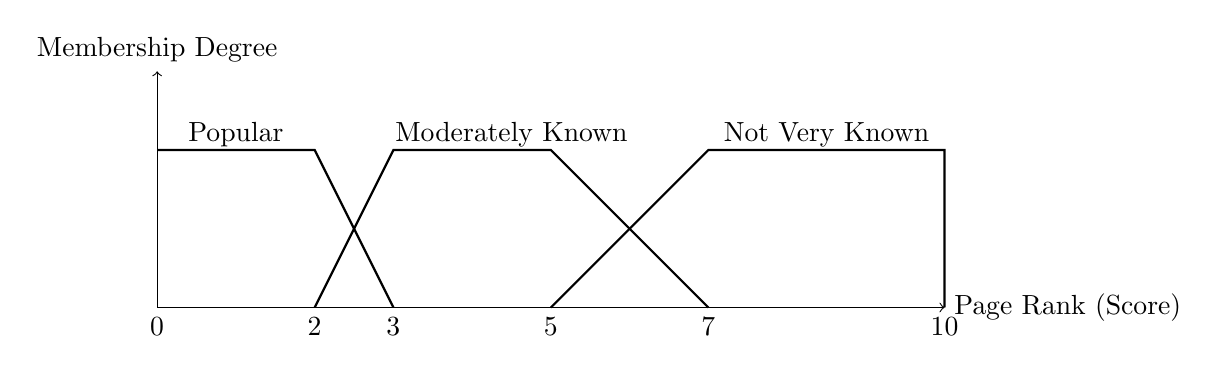
\begin{tikzpicture}
    % Axis
    \draw[->] (0,0) -- (10,0) node[right] {Page Rank (Score)};
    \draw[->] (0,0) -- (0,3) node[above] {Membership Degree};

    % Popular
    \draw[thick] (0,2) -- (2,2) -- (3,0);
    \node at (1,2.2) {Popular};

    % Moderately Known
    \draw[thick] (2,0) -- (3,2) -- (5,2) -- (7,0);
    \node at (4.5,2.2) {Moderately Known};

    % Not Very Known
    \draw[thick] (5,0) -- (7,2) -- (10,2) -- (10,0);
    \node at (8.5,2.2) {Not Very Known};

    % Labels
    \node[below] at (0,0) {0};
    \node[below] at (2,0) {2};
    \node[below] at (3,0) {3};
    \node[below] at (5,0) {5};
    \node[below] at (7,0) {7};
    \node[below] at (10,0) {10};
\end{tikzpicture}
\caption{Membership Functions for Page Rank}
\label{fig:membership_page_rank}
\end{figure}

\subsection{Output Linguistic Variable}

The output variable measures the phishing risk of a website, ranging from 0 to 100 percent. We define four fuzzy categories: safe, weakly suspicious, strongly suspicious, and phishing. Each category is represented by a trapezoidal membership function.

\begin{table}[H]
\centering
\begin{tabularx}{\textwidth}{|>{\hsize=0.7\hsize}X|>{\hsize=0.6\hsize}X|>{\hsize=1.7\hsize}X|}
\hline
\textbf{Fuzzy Category} & \textbf{Range} & \textbf{Argumentation} \\
\hline
Safe & [0, 0, 15, 25] & Indicates a very low risk of phishing. Websites in this category are considered safe and trustworthy. \\
\hline
Weakly Suspicious & [15, 25, 35, 45] & Suggests a low risk of phishing. These websites may have some minor issues but are generally considered safe. \\
\hline
Strongly Suspicious & [45, 55, 65, 75] & Represents a moderate risk of phishing. Websites in this category exhibit several suspicious characteristics and warrant caution. \\
\hline
Phishing & [65, 75, 100, 100] & Indicates a high risk of phishing. Websites in this category are highly likely to be phishing sites and should be avoided. \\
\hline
\end{tabularx}
\caption{Fuzzy Categories for Phishing Risk}
\label{tab:phishing_risk}
\end{table}

\begin{figure}[H]
\centering
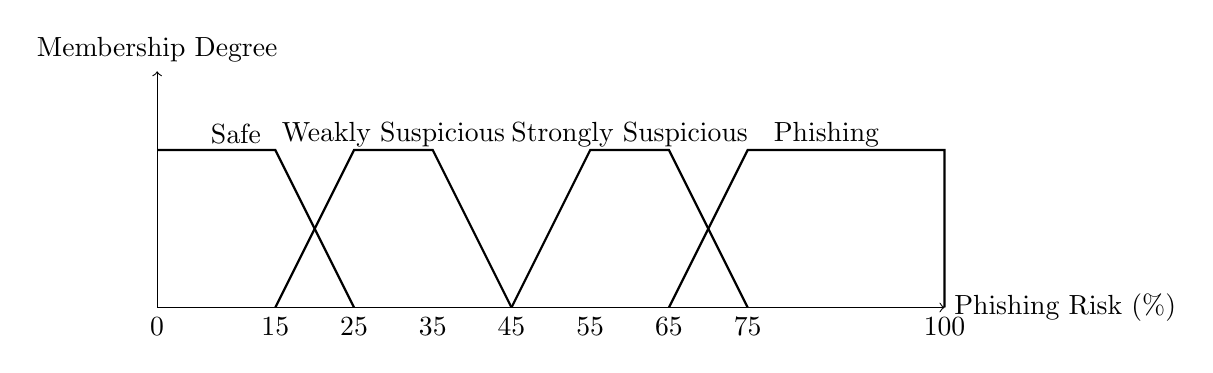
\begin{tikzpicture}
    % Axis
    \draw[->] (0,0) -- (10,0) node[right] {Phishing Risk (\%)};
    \draw[->] (0,0) -- (0,3) node[above] {Membership Degree};

    % Safe
    \draw[thick] (0,2) -- (1.5,2) -- (2.5,0);
    \node at (1,2.2) {Safe};

    % Weakly Suspicious
    \draw[thick] (1.5,0) -- (2.5,2) -- (3.5,2) -- (4.5,0);
    \node at (3,2.2) {Weakly Suspicious};

    % Strongly Suspicious
    \draw[thick] (4.5,0) -- (5.5,2) -- (6.5,2) -- (7.5,0);
    \node at (6,2.2) {Strongly Suspicious};

    % Phishing
    \draw[thick] (6.5,0) -- (7.5,2) -- (10,2) -- (10,0);
    \node at (8.5,2.2) {Phishing};

    % Labels
    \node[below] at (0,0) {0};
    \node[below] at (1.5,0) {15};
    \node[below] at (2.5,0) {25};
    \node[below] at (3.5,0) {35};
    \node[below] at (4.5,0) {45};
    \node[below] at (5.5,0) {55};
    \node[below] at (6.5,0) {65};
    \node[below] at (7.5,0) {75};
    \node[below] at (10,0) {100};
\end{tikzpicture}
\caption{Membership Functions for Phishing Risk}
\label{fig:membership_phishing_risk}
\end{figure}

\section{Task 2: Definition of the Rule Base}

% Define a set of conjunctive rules for the fuzzy expert system.
% - Decide appropriate premises for each rule.
% - Assign a degree of support to each rule.
% - Ensure rules cover all possible combinations of input values.
% - Use rules of different lengths.
% - Avoid inconsistencies and overlaps in the rules.
% - Limit the number of rules to 30-35 for manageability.

\subsection{Rule Development}

% Discuss the methodology used to develop the rules.
% Explain how evidence from literature supports the rule definitions. -> Need references

\subsection{Complete Rule Set}

WORK IN PROGRESS, THIS COMPLETE RULE SET IS NOT FINAL

\begin{table}[H]
\centering
\footnotesize
\setlength{\extrarowheight}{1pt}
\begin{tabularx}{\textwidth}{|>{\centering\arraybackslash}p{0.04\textwidth}|>{\raggedright\arraybackslash}p{0.12\textwidth}|>{\raggedright\arraybackslash}p{0.12\textwidth}|>{\raggedright\arraybackslash}p{0.15\textwidth}|>{\raggedright\arraybackslash}p{0.12\textwidth}|>{\raggedright\arraybackslash}p{0.13\textwidth}|>{\raggedright\arraybackslash}p{0.12\textwidth}|}
\hline
\rowcolor{gray!30}
\textbf{\#} & \textbf{Null Links} & \textbf{Ext. CSS} & \textbf{Domain Reg.} & \textbf{Traffic} & \textbf{Page Rank} & \textbf{Risk} \\ \hline
\textbf{1}  & High      & Very Few & Short  & Very Low    & Not very known   & Very High     \\\rowcolor{lightgray}
\textbf{2}  & High      & Few      & Short  & Low         & Not very known   & Very High     \\
\textbf{3}  & High      & Normal   & Short  & Moderate    & Not very known   & Very High     \\\rowcolor{lightgray}
\textbf{4}  & High      & Very Few & Medium & Low         & Moderately known & High          \\
\textbf{5}  & High      & Few      & Medium & Moderate    & Moderately known & High          \\\rowcolor{lightgray}
\textbf{6}  & High      & Normal   & Medium & High        & Moderately known & High          \\
\textbf{7}  & High      & Very Few & Long   & Moderate    & Popular          & Moderate      \\\rowcolor{lightgray}
\textbf{8}  & High      & Few      & Long   & High        & Popular          & Moderate      \\
\textbf{9}  & High      & Normal   & Long   & High        & Popular          & Moderate      \\\rowcolor{lightgray}
\textbf{10} & Moderate  & Very Few & Short  & Very Low    & Not very known   & High          \\
\textbf{11} & Moderate  & Few      & Short  & Low         & Not very known   & High          \\\rowcolor{lightgray}
\textbf{12} & Moderate  & Normal   & Short  & Moderate    & Not very known   & High          \\
\textbf{13} & Moderate  & Very Few & Medium & Low         & Moderately known & Moderate      \\\rowcolor{lightgray}
\textbf{14} & Moderate  & Few      & Medium & Moderate    & Moderately known & Moderate      \\
\textbf{15} & Moderate  & Normal   & Medium & High        & Moderately known & Moderate      \\\rowcolor{lightgray}
\textbf{16} & Moderate  & Very Few & Long   & Moderate    & Popular          & Low           \\
\textbf{17} & Moderate  & Few      & Long   & High        & Popular          & Low           \\\rowcolor{lightgray}
\textbf{18} & Moderate  & Normal   & Long   & High        & Popular          & Low           \\
\textbf{19} & Low       & Very Few & Short  & Very Low    & Not very known   & Moderate      \\\rowcolor{lightgray}
\textbf{20} & Low       & Few      & Short  & Low         & Not very known   & Moderate      \\
\textbf{21} & Low       & Normal   & Short  & Moderate    & Not very known   & Moderate      \\\rowcolor{lightgray}
\textbf{22} & Low       & Very Few & Medium & Low         & Moderately known & Low           \\
\textbf{23} & Low       & Few      & Medium & Moderate    & Moderately known & Low           \\\rowcolor{lightgray}
\textbf{24} & Low       & Normal   & Medium & High        & Moderately known & Low           \\
\textbf{25} & Low       & Very Few & Long   & Moderate    & Popular          & Very Low      \\\rowcolor{lightgray}
\textbf{26} & Low       & Few      & Long   & High        & Popular          & Very Low      \\
\textbf{27} & Low       & Normal   & Long   & High        & Popular          & Very Low      \\\rowcolor{lightgray}
\textbf{28} & High      & Very Few & Short  & High        & Not very known   & Very High     \\
\textbf{29} & Moderate  & Few      & Medium & Very Low    & Moderately known & High          \\\rowcolor{lightgray}
\textbf{30} & Low       & Normal   & Long   & Very Low    & Popular          & Low           \\
\textbf{31} & High      & Few      & Medium & Very Low    & Not very known   & Very High     \\\rowcolor{lightgray}
\textbf{32} & Moderate  & Normal   & Short  & High        & Moderately known & High          \\
\textbf{33} & Low       & Very Few & Medium & Very Low    & Moderately known & Moderate      \\\rowcolor{lightgray}
\textbf{34} & High      & Normal   & Long   & Low         & Popular          & Moderate      \\
\textbf{35} & Low       & Few      & Short  & High        & Not very known   & Moderate      \\
\hline
\end{tabularx}
\caption{Complete Rule Set for Phishing Detection}
\label{tab:complete_rule_set}
\end{table}


\section{Task 3: Implementation Using MATLAB Fuzzy Toolkit}

% Describe the implementation of the fuzzy expert system in MATLAB.
% - Specify the use of min as t-norm and max as t-conorm.
% - Use Center of Area for defuzzification.
% Validate the system using 3D plots of the rules.

\subsection{System Configuration}

% Explain how the fuzzy inference system was set up in MATLAB.
% Include screenshots if necessary.

\subsection{Validation}

% Present the 3D plots.
% Discuss how they validate the system's behavior.

\section{Task 4: Testing the System}

% Test the fuzzy expert system with four different websites.
% - Select or invent appropriate test cases representing different situations.
% - Ensure some cases activate more than one label of the same variable.
% Report the results with explanations and screenshots.

\subsection{Test Cases}

% Describe each test case in detail.
% Include input values and expected outcomes.

\subsection{Results and Discussion}

% Present the outputs of the system for each test case.
% Show activations of rules and explain the results.

\section{Task 5: Design of an Enhanced Fuzzy Expert System}

% Question: How to visualize this?
% Propose a design for a more comprehensive fuzzy expert system.
% - Include more features about websites.
% - Illustrate inputs, outputs, and rule blocks in a diagram.
% Note: No specific variable definitions or rules are required.

\subsection{Proposed System Architecture}

% Describe the proposed enhancements and their benefits.
% Include a figure illustrating the system.

\section{Conclusion}

% Summarize the work done.
% Reflect on the effectiveness of the fuzzy expert system.
% Discuss potential improvements and future work.

% \appendix

\printbibliography

\end{document}